%%%%%%%%%%%%%%%%%%%%%%%%%%%%%%%%%%%%%%%%%%%%%%%%%%%%%%%%%%%%
%%  This Beamer template was created by Cameron Bracken.

\documentclass[xcolor=x11names,compress, aspectratio=169]{beamer}
%\documentclass[xcolor=x11names,compress, handhouts, aspectratio=169]{beamer}
%% General document
\usepackage{graphicx, subfig}
%% Beamer Layout
\useoutertheme[subsection=false,shadow]{miniframes}
\useinnertheme{default}
\usefonttheme{serif}
\usepackage{palatino}

%%%%%%% Mes Packages %%%%%%%%%%%%%%%%
%\usepackage[french]{babel}
\usepackage[T1]{fontenc}
\usepackage{color}
\usepackage{xcolor}
\usepackage{dsfont} % Pour indicatrice
\usepackage{url}
\usepackage{multirow}
%remove the icon
\setbeamertemplate{bibliography item}{}

%remove line breaks
\setbeamertemplate{bibliography entry title}{}
\setbeamertemplate{bibliography entry location}{}
\setbeamertemplate{bibliography entry note}{}

%% ------ MEs couleurs --------
\definecolor{vert}{rgb}{0.1,0.7,0.2}
\definecolor{brique}{rgb}{0.7,0.16,0.16}
\definecolor{twitterblue}{rgb}{0, 0.42, 0.58}
\definecolor{airforceblue}{rgb}{0.36, 0.54, 0.66}
\definecolor{siap}{RGB}{3,133, 200}
\definecolor{grey}{rgb}{0.52, 0.52, 0.51}
\definecolor{gris}{rgb}{0.7, 0.75, 0.71}


%%%%%%%%%%%%%%%%% BEAMER PACKAGE %%%%%%%


\setbeamercolor{itemize item}{fg=siap}
%\setbeamercolor{itemize subitem}{fg=blue}
%\setbeamercolor{itemize subsubitem}{fg=cyan}


\setbeamerfont{title like}{shape=\scshape}
\setbeamerfont{frametitle}{shape=\scshape}

\setbeamercolor*{lower separation line head}{bg=DeepSkyBlue4}
\setbeamercolor*{normal text}{fg=black,bg=white}
\setbeamercolor*{alerted text}{fg=siap}
\setbeamercolor*{example text}{fg=black}
\setbeamercolor*{structure}{fg=black}
\setbeamercolor*{palette tertiary}{fg=black,bg=black!10}
\setbeamercolor*{palette quaternary}{fg=black,bg=black!10}

% Set the header color to SIAP's color
\setbeamercolor*{frametitle}{fg=siap}

\renewcommand{\(}{\begin{columns}}
\renewcommand{\)}{\end{columns}}
\newcommand{\<}[1]{\begin{column}{#1}}
\renewcommand{\>}{\end{column}}


%% Add footer with logo
\setbeamertemplate{footline}{%
  \begin{beamercolorbox}[wd=\paperwidth,ht=2.5ex,dp=1.125ex,%
    leftskip=.3cm,rightskip=.3cm plus1fil]{author in head/foot}
    
\includegraphics[height=4ex]{SIAP_logo_Big.png}\hfill
    \insertshortauthor\hfill\insertshorttitle\hfill  \textcolor{siap}{\textit{\insertframenumber}}
  \end{beamercolorbox}%
}


% Path for the graphs
\graphicspath{{Graphics/}
{../../../../Visualisation/Presentations/Graphics/}
{../../Visualisation/Presentations/Graphics/}
{c:/Gitmain/MLCourse/UNML/Module0/M0_files/figure-html/}
{c:/Chris/UN-ESCAP/MyCourses2022/MLOS2022/Slides/Graphics/}
{c:/Chris/UN-ESCAP/MyCourses2023/BigDataKostat/Slides/Graphics/}
 }

%remove navigation symbols
\setbeamertemplate{navigation symbols}{}


% Natbib for clean bibliography
\usepackage[comma,authoryear]{natbib}

%%%% Use it or not %%%%

\title{\textcolor{siap}{Big Data and Data Science for Gender Statistics in Asia and the Pacific}}
\subtitle{}
\author{\textcolor{grey}{Christophe Bontemps}}
\institute{\large{\emph{Statistical Institute for Asia and the Pacific} } \\
    
\includegraphics[height=10ex]{SIAP_logo_Big.png}}
\date{}

%%%%%

\title{\textcolor{siap}{Big Data and Data Science for Gender Statistics in Asia and the Pacific \\ \vspace{0.5cm} }}

\subtitle{\textcolor{brique}{\Large{Principles of Machine Learning }}}
\author{Christophe Bontemps}
\institute{ 
\includegraphics[height=10ex]{SIAP_logo_Big.png}}
\date{}

\begin{document}

\section{Motivation}

\begin{frame}
  \titlepage
\end{frame}


\begin{frame} % Cover slide
\frametitle{\textcolor{brique}{[-  \textbf{Agenda} -]}}
\begin{itemize}[<+-|alert@+>]
   \item Why Machine learning is useful for Big Data
   \item[$\hookrightarrow$] Example with Regression
   \item Statistical learning \textit{vs} Machine Learning
   \item Cross-Validation at the core of ML
   \item Q\&A
\end{itemize}
\end{frame}

%%%%%%%%%%%%%%%%%%%%%%%%%%%%%%%%% AI %%%%%%

\section{ML for Big Data}

\begin{frame}{Why Machine Learning for Big Data?}

\pause

\begin{itemize}[<+->]
    \item What is Machine Learning used for?
    \item "\emph{ML can unlock the potential of big data and derive meaningful insights}"
    \item[$\hookrightarrow$] How?
    \item ML embeds \emph{classification}, \emph{regression}, \emph{clustering}, \emph{non-linear modeling}
    \item[$\hookrightarrow$] Predictions
    \item ML algorithms are  \textbf{scalable} and can be \textbf{parallelized}
    \item[$\hookrightarrow$] ML is almost always used in any Big Data application

\end{itemize}
\end{frame}

%%%%%%%%%%%%%%%%%%%%%%%%   AI  %%%%%%%


%\section{Statistical  learning}
%
%
%%%% Title page %%%%%
%\begin{frame}
%\Large{ \color{siap}{Module 2 - Machine Learning }}
%
%\hspace{1cm}
%
%\color{brique}{\huge{Statistical learning: \\ \textit{vs} Machine Learning }}
%
%\hspace{2cm}
%\begin{center}
%
%
\includegraphics[height=0.10\textwidth]{SIAP_logo_Big.png}
%
%\end{center}
%\end{frame}
%
%
%
%\begin{frame} % Cover slide
%\frametitle{What Is Statistical Learning?}
%\pause
%\begin{itemize}[<+->]
%\item[]
%\begin{center}
%\emph{`` Statistical learning refers to a vast set of tools for understanding data''}\\
%
%{\scriptsize Gareth James,  Daniela Witten, Trevor Hastie ,  Robert Tibshirani (2021)}\\
%\vspace{0.5cm}
%\end{center}
%\pause
%   \only<4-7>{$\hookrightarrow$ Involves building statistical models\\ }
%   \only<5> { $\hookrightarrow$ Goals are estimation or prediction \\ }
%   \only<6> { $\hookrightarrow$ Goals are \textbf{estimation} or prediction \\ }
%   \only<7> {$\hookrightarrow$ Goals are estimation or \textbf{prediction} \\ }
% \end{itemize}
%\end{frame}
%
%


\section{Learning}

\begin{frame} % Cover slide
\frametitle{Relating $x$ and $y$ }
 \begin{itemize}
  \item<+->[] 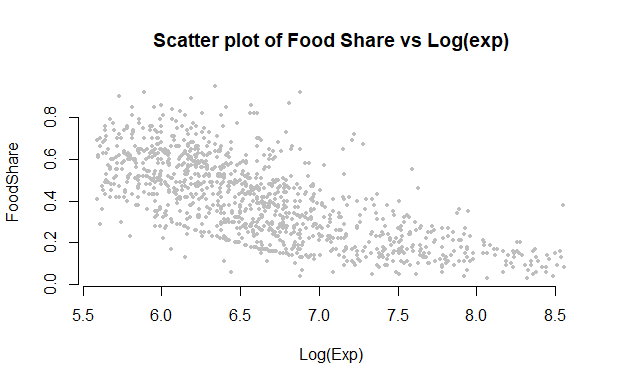
\includegraphics[width = 0.7\textwidth]{M0-Scatter-1.png}
  \item<+->[]  Interest in the \textbf{relationship} between $x$ and $y$ ,  \emph{i.e.} \textbf{$ y = f(x)$}
 \end{itemize}
\end{frame}


%\begin{frame} % Cover slide
%\frametitle{Understanding = estimate $f(\cdot)$ }
% \begin{itemize}
%  \item<+->[] 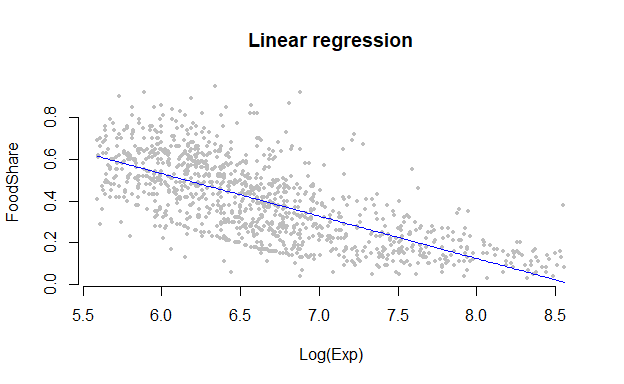
\includegraphics[width = 0.7\textwidth]{M0-Scatter-lm-1.png}
%  \item<+->[]  $f(\cdot)$ is the regression line
% \end{itemize}
%\end{frame}


\begin{frame} % Cover slide
\frametitle{Why estimating $f(x)$?}

\pause

 \begin{itemize}
  \item<+-> Inference
   \begin{itemize}
  \item<+->[] \textit{Understand} the nature of the relationship between $X$ and $Y$
  \item<+->[] \textit{Identify}  "important" variables to understand $Y$
 \end{itemize}
  \item<+-> Prediction
   \begin{itemize}
  \item<+->[] Predict $y$ for any \textbf{new} $x$ using $f(\cdot)$
 \end{itemize}
 \item<+-> In practice we must estimate  $f(\cdot)$ using a model:
 \item<+->[] $$ y = f(x) + \varepsilon $$
 \item<+->[] We denote by $\widehat{f(\cdot)}$ the estimate of $f(\cdot)$
 \end{itemize}
\end{frame}


\begin{frame} % Cover slide
\frametitle{How to estimate $f(\cdot)$?}
 \begin{itemize}
  \item<+-> Parametric methods
   \begin{itemize}[<+->]
      \item[] Specify a form for $f(\cdot)$, for example linear:
      \item[] $$y = \beta_0 + \beta_1 x_ + \varepsilon$$
      \item Let's play: Find the line that "fits" the data...
      \item[]  \href{https://xtophedataviz.shinyapps.io/RegressionApp/}{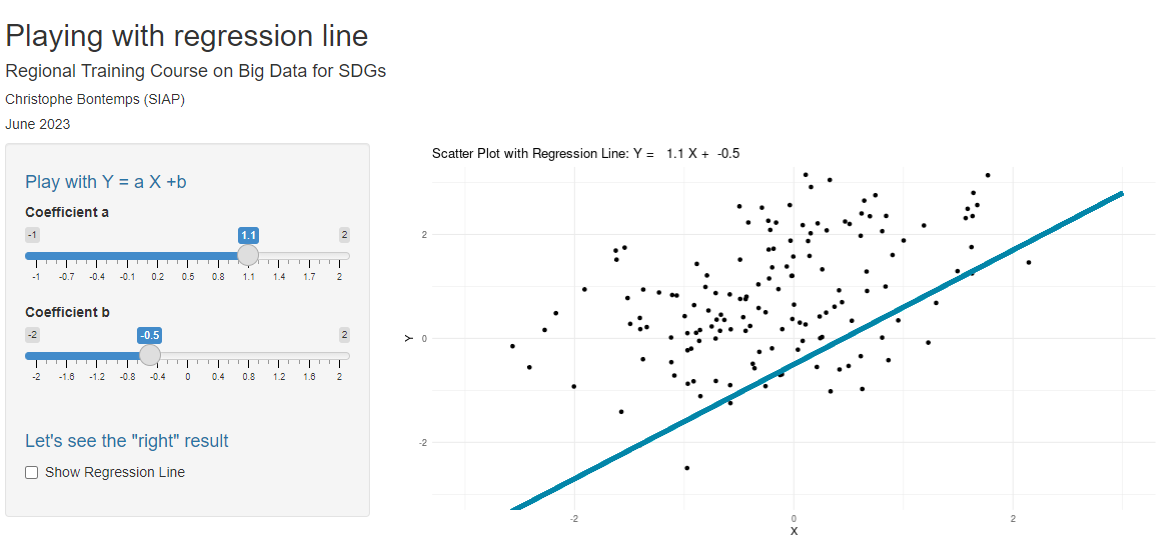
\includegraphics[width = 0.6\textwidth]{RegressionLineGame.PNG}}
 \end{itemize}
 \end{itemize}
\end{frame}



\begin{frame} % Cover slide
\frametitle{How to estimate $f(\cdot)$?}
 \begin{itemize}
  \item<+-> Parametric methods
   \begin{itemize}
      \item<+->[] Specify a form for $f(\cdot)$, for example linear:
      \item<+->[] $$y = \beta_0 + \beta_1 x_ + \varepsilon$$
      %\item<+-> The problem is then to estimate $ \beta_0$ and $\beta_1 \; \hookrightarrow $ ($\widehat \beta_0, \widehat \beta_1$  are the estimates)
      \item<+-> The goal is to find the line that is  \textbf{minimizing} the distance to the observed points $(x_i, y_i)$.
                The distance is computed as the Mean Square Error (MSE): $$ MSE(\beta_0, \beta_1) = \frac{1}{n} \sum_{i=1}^{n} \bigl(y_i - (\beta_0 + \beta_1 x_i)\bigr)^2 $$
      \item<+-> The regression line, defined by $\beta_0$ and $\beta_1$,  is simply the solution of:
       $$Min_{\; (\beta_0 , \beta_1)} \; MSE(\beta_0, \beta_1) $$
   \end{itemize}
 \item<+->[]  The MSE it is the \textit{cost function} minimized to determine $ (\widehat \beta_0, \widehat \beta_1)$
 \end{itemize}

\end{frame}


\begin{frame} % Cover slide
\frametitle{How to estimate $f(\cdot)$: In practice}
 \begin{itemize}
  \item<+->[] 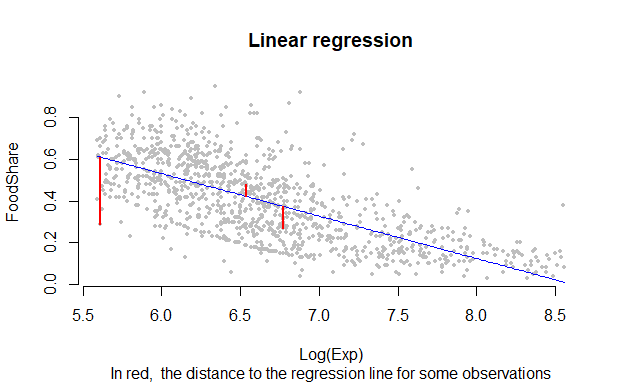
\includegraphics[width = 0.7\textwidth]{M0-scatter-Regline-1.png}
  \item<+->[] The \href{https://mlu-explain.github.io/linear-regression/}{\textcolor[rgb]{0.00,0.50,0.75}{regression line}} is found by minimizing the sum of all distances or \textbf{MSE}
 \end{itemize}
\end{frame}


\begin{frame} % Cover slide
\frametitle{Results: $ \widehat{f(\cdot)}$}
From the result and the estimated  parameters $ (\widehat \beta_0, \widehat \beta_1)$, we see that there is a relation, and that it is decreasing.
\begin{table}
\centering
\begin{tabular}{l|rrrc}
\hline
  & Estimate & Std. Error & t value & $Pr(>|t|)$\\
\hline
(Intercept) & 1.75 & 0.04 & 41.09 & 0\\
\hline
ltexp &\textbf{ $-0.20^{***}$ }& 0.01 & -31.84 & 0\\
\hline
\end{tabular}
\end{table}
\vspace{0.5cm}
 The quality of the adjustment may be measured by the $R^2$ = 0.478

\end{frame}



\section{Machine learning}

%
%\begin{frame}
%\frametitle{\textcolor{brique}{Statistical \textit{vs} Machine Learning}}
%What is the goal?
%\pause
%\begin{itemize}[<+->]
%\item If the goal is to formalize a model, one may focus on testing statistical properties, significance, relationships, ...
%\item[] $\hookrightarrow $ this is the purpose of \textbf{Statistical Learning }
%\item If the goal is to predict, one may focus on prediction accuracy
%\item[] $\hookrightarrow $ this is the purpose of \textbf{Machine Learning }
%\item Many statistical learning methods are relevant and useful to estimate $f(\cdot)$
%\item In practice we'll use both tools to  "\emph{understand the data}"
%%\item $f(\cdot)$ can take continuous (regression) or discrete values (classification)
%%\item Choosing the best method is difficult
%
%\end{itemize}
%\end{frame}


\begin{frame}
\frametitle{\textcolor{brique}{ What \emph{learning} means?}}
The classical approach
\begin{itemize}[<+->]
\item For regression we estimate $f(\cdot)$ on \textbf{the whole data set}
\item[] 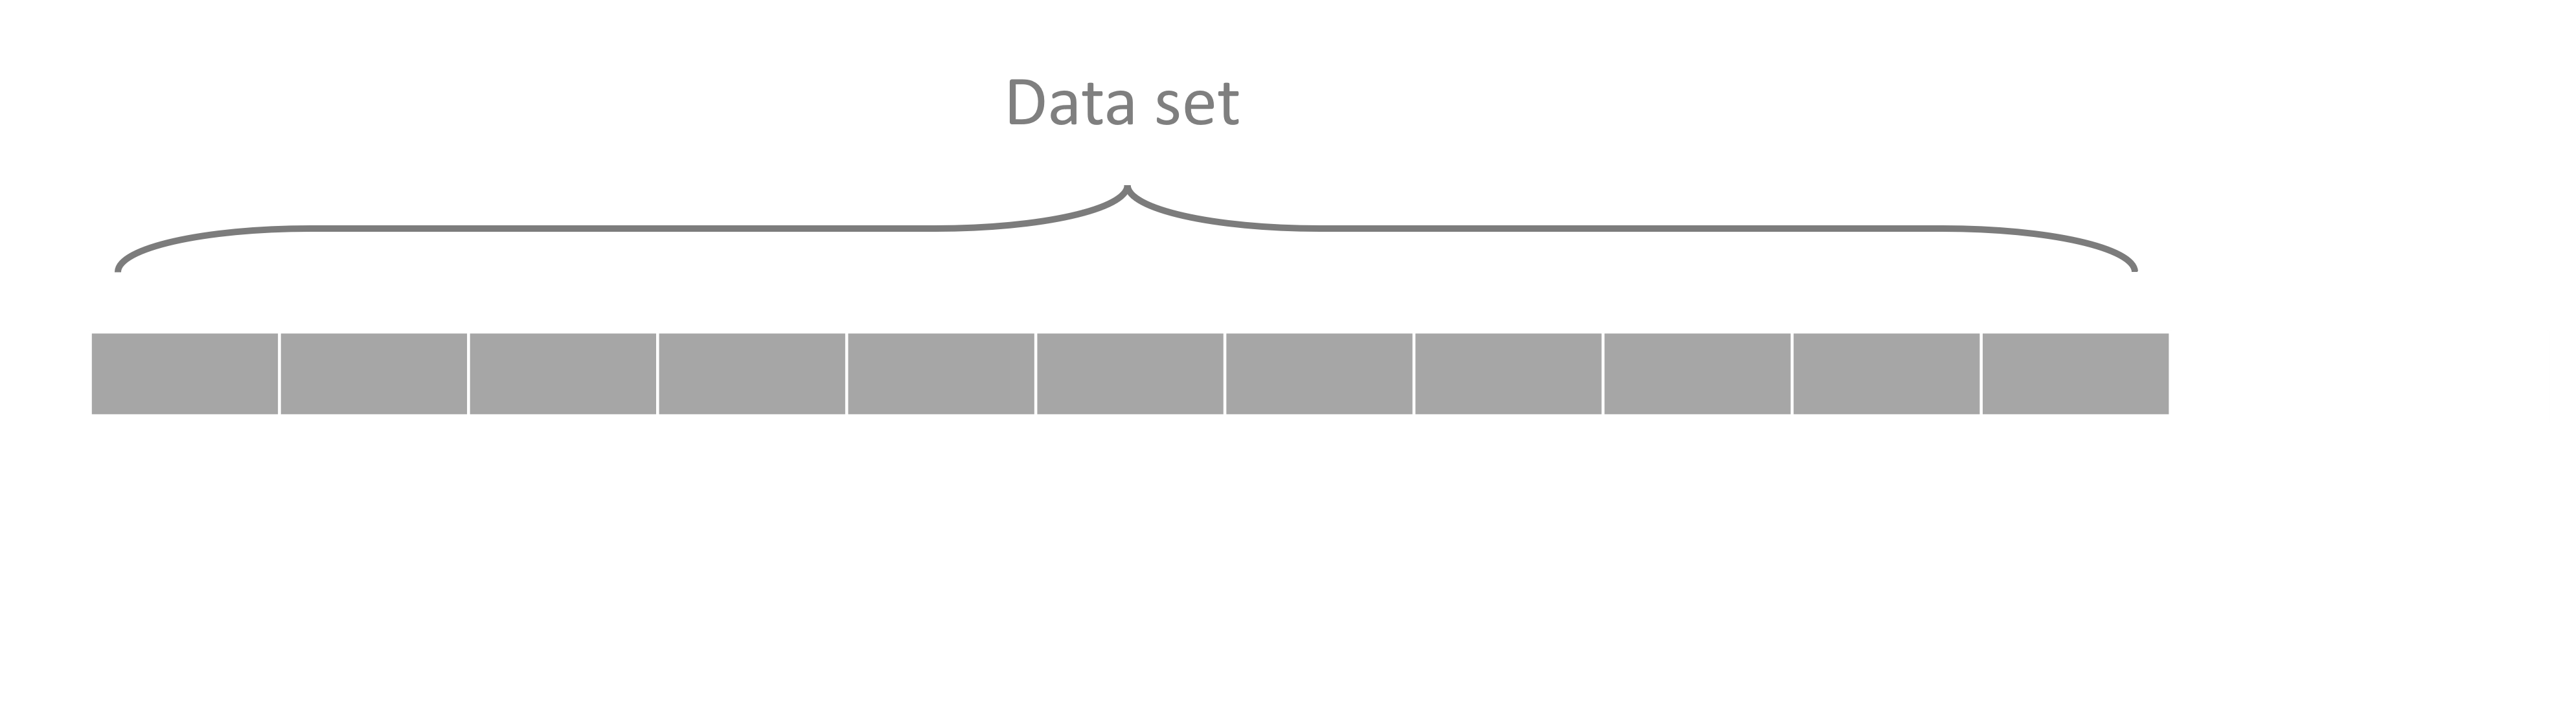
\includegraphics[width = 0.8\textwidth]{ML-Sets1.png}
\item We have estimated $f(\cdot)$ by $\widehat f(\cdot)$  and minimized some cost function
% such as the
%$ MSE =  \frac{1}{n} \; \sum_ {i=1}^n \bigl( y_i - \widehat f(x_i) \bigr)^2 $
\item The data serve \textbf{both} for estimating $f(\cdot)$ \textbf{and} computing the prediction error
\item \emph{Will that function predict well on a \textcolor[rgb]{1.00,0.00,0.00}{\textbf{new }}sample?}
\end{itemize}
\end{frame}

\section{Cross-Validation}

\begin{frame} % Cover slide
\frametitle{Cross Validation}
\begin{columns}[t]
 \begin{column}{0.7\textwidth}
 \begin{itemize}[<+->]
    \item Imagine you use a linear model on a data set:  $$y = \beta_0 + \beta_1 x_ + \varepsilon$$
    \item  Is it good for predicting?
    \item Is it better than a quadratic model? $y = \beta_0 + \beta_1 x_ + + \beta_2 x^2+ \varepsilon$
    \item[$\hookrightarrow$] How could we know how good/bad it is?
    \item Let's play:  \emph{Manual} Cross-validation!
    \item[]  \href{https://xtophedataviz.shinyapps.io/MLRegressionExample/}{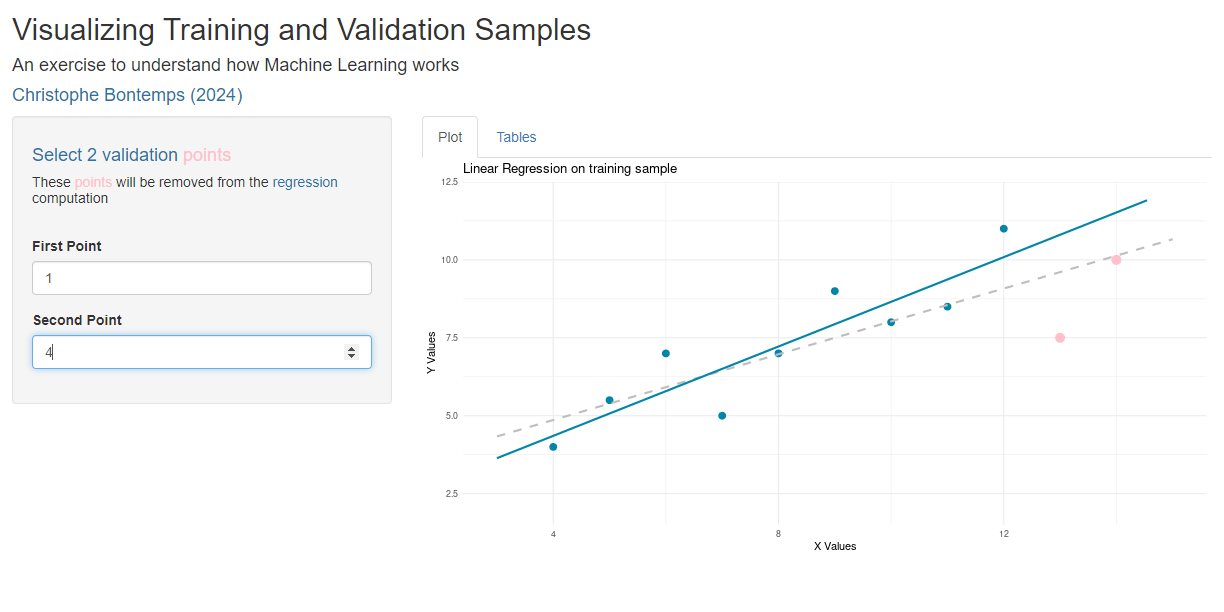
\includegraphics[width = 0.6\textwidth]{CrossValidationRegression.png}}
 \end{itemize}
 \end{column}
    \begin{column}{0.5\textwidth}
       \begin{itemize}
        \item[] 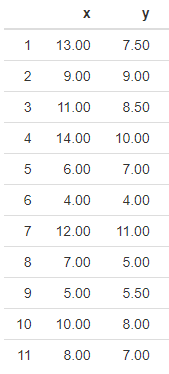
\includegraphics[width = 0.4\textwidth]{Dataset.png}
       \end{itemize}
    \end{column}
\end{columns}
\end{frame}


\begin{frame}
\frametitle{\textcolor{brique}{ What \emph{learning} means?}}
The classical approach (again)
\begin{itemize}
\item Estimating $f(\cdot)$ on \textbf{the whole data set} is not enough for prediction.
\item[] 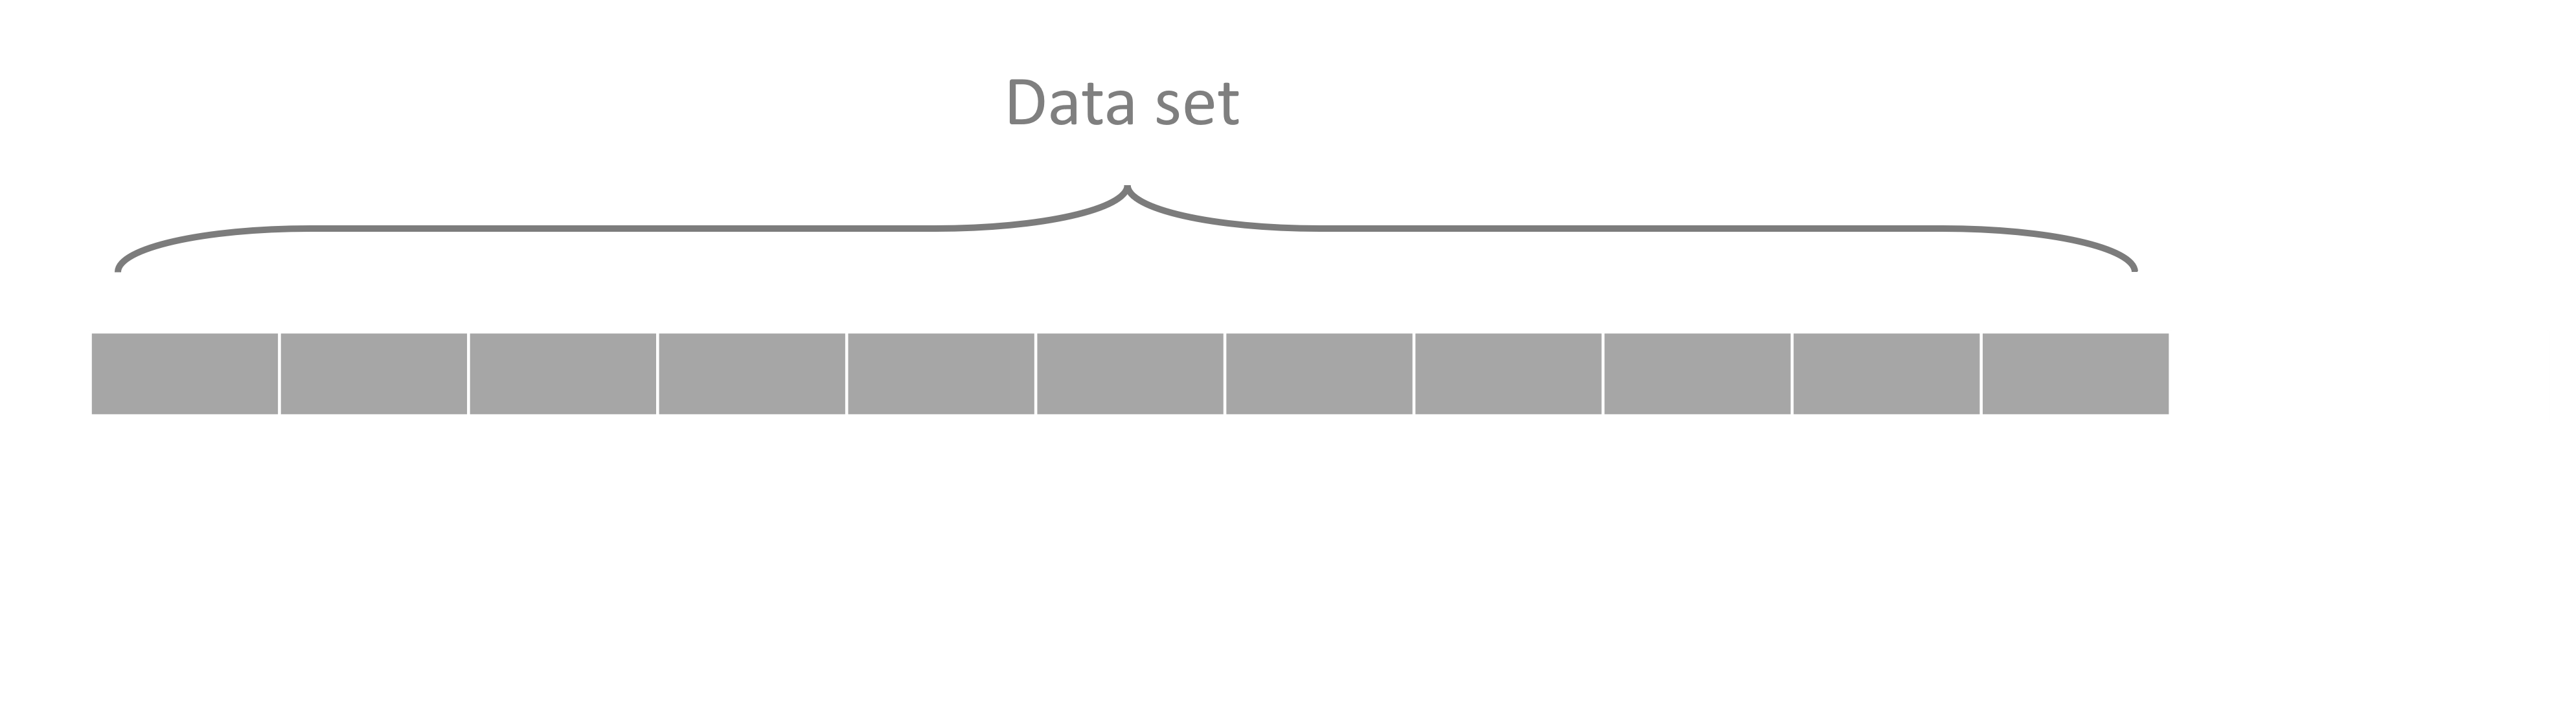
\includegraphics[width = 0.8\textwidth]{ML-Sets1.png}
\item  $\widehat f(\cdot)$  minimizes some cost function on \textbf{the whole data set}
%\item The data serve \textbf{both} for estimating $f(\cdot)$ \textbf{and} computing the prediction error
\item \emph{Will that estimate be good on a \textcolor[rgb]{1.00,0.00,0.00}{\textbf{new }} \emph{unseen} sample?}
\end{itemize}
\end{frame}


\begin{frame}
\frametitle{\textcolor{brique}{ What learning means?}}
A different approach: \textit{resampling}
\begin{itemize}[<+->]
\item Our goal is  evaluate the prediction accuracy of $\widehat f(\cdot)$ on a new, \textbf{unseen}, data set
\item Since we may not have \textbf{unseen} data, we will construct one
\item[] 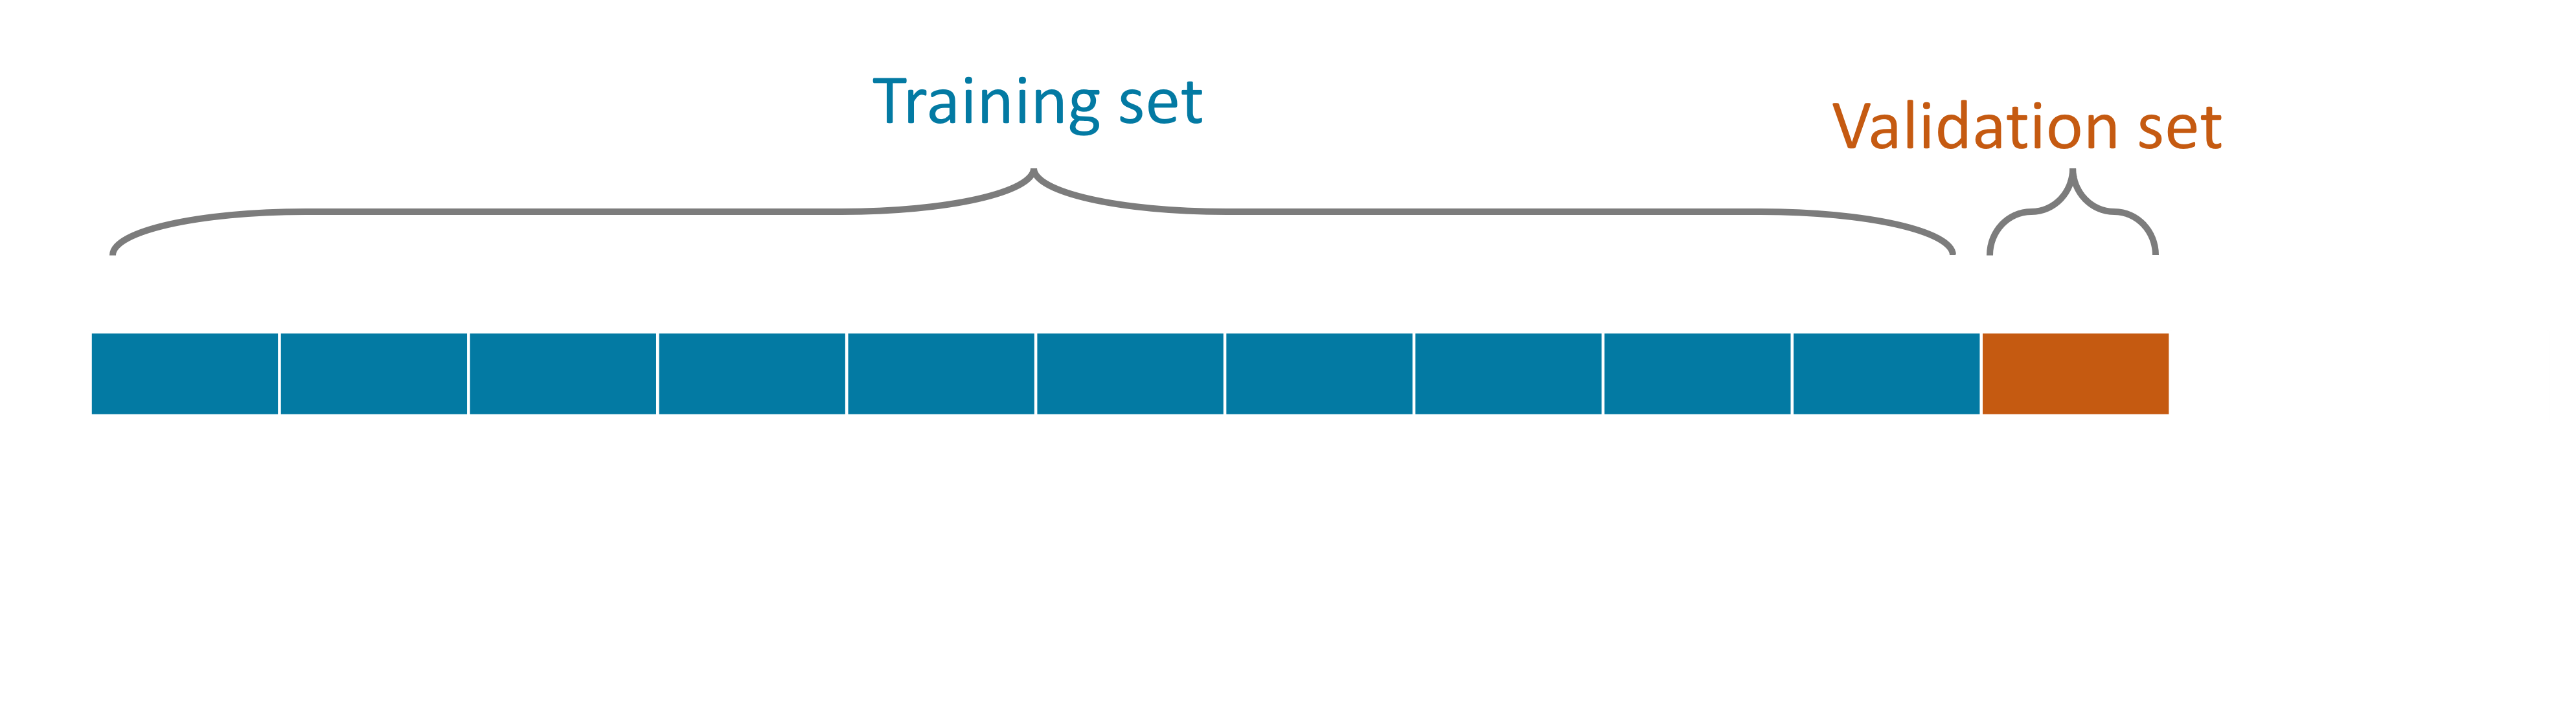
\includegraphics[width = 0.8\textwidth]{ML-Sets4.png}
\item Compare $y_i$  with the prediction based on the validation set $x$s
\end{itemize}
\end{frame}



\begin{frame}
\frametitle{\textcolor{brique}{Why different sets? }}
Estimating parameters using predictions accuracy
\begin{itemize}[<+->]
\item When estimating $f(\cdot)$ on the whole data set, over-fitting may occur
\item The validation set provides a good way to evaluate the prediction capabilities of a model and the prediction error on a new data set
\item[] 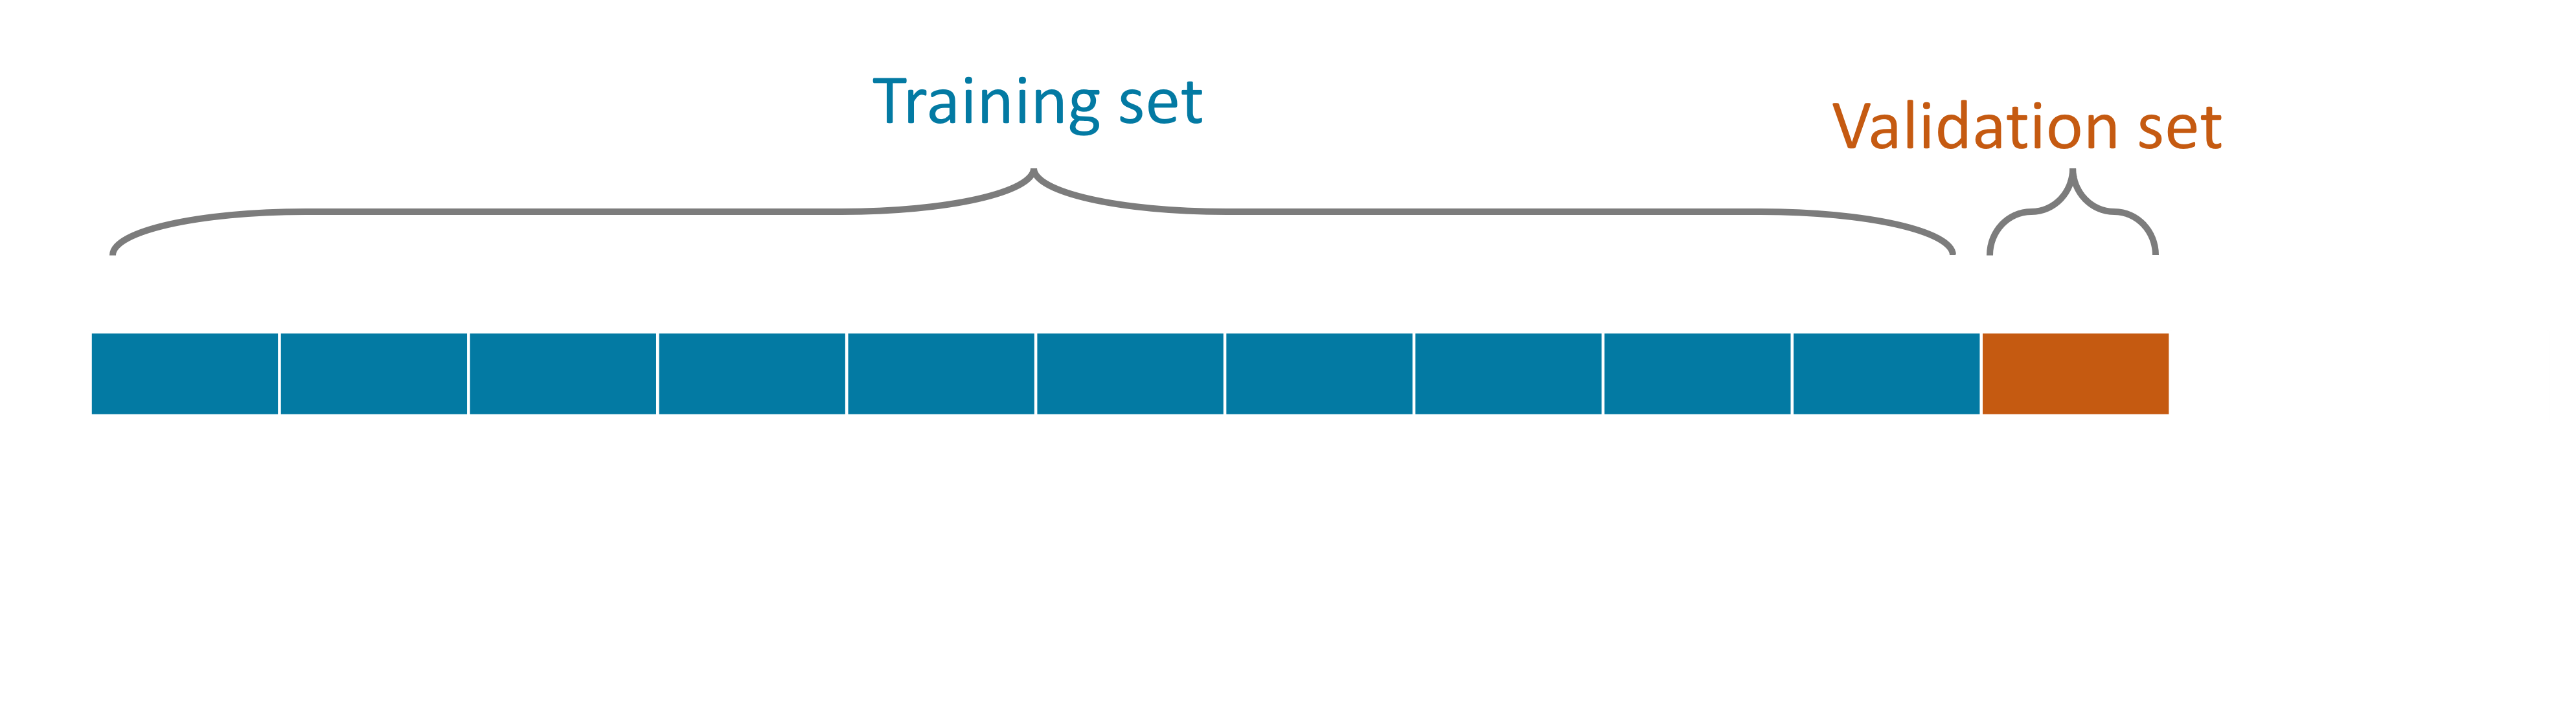
\includegraphics[width = 0.8\textwidth]{ML-Sets4.png}
\item Prediction accuracy (using $\widehat f(\cdot)$) is then evaluated on the validation set \textbf{only}
\end{itemize}
\end{frame}


\begin{frame}
\frametitle{\textcolor{brique}{Constructing training \& validation sets}}
In practice, the validation set is not a block
\begin{itemize}[<+->]
\item[] 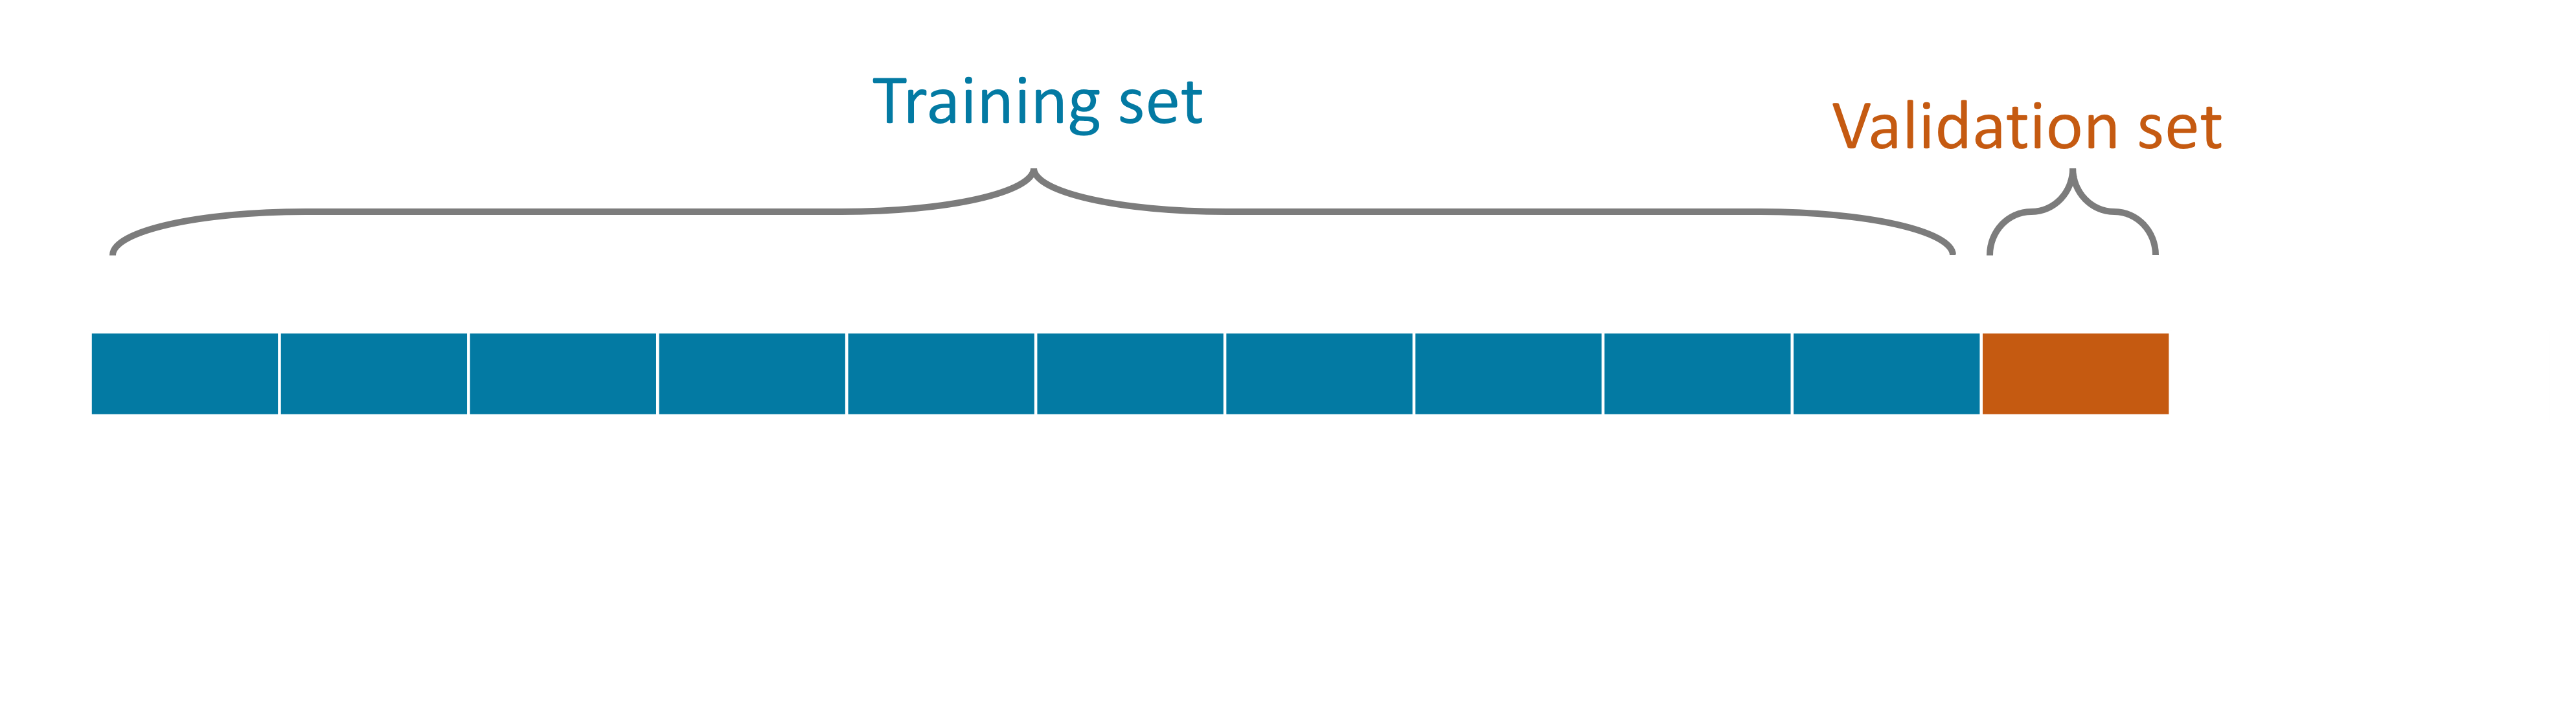
\includegraphics[width = 0.8\textwidth]{ML-Sets4.png}
\item The validation set is constructed from a randomly drawn observations.
\item[] 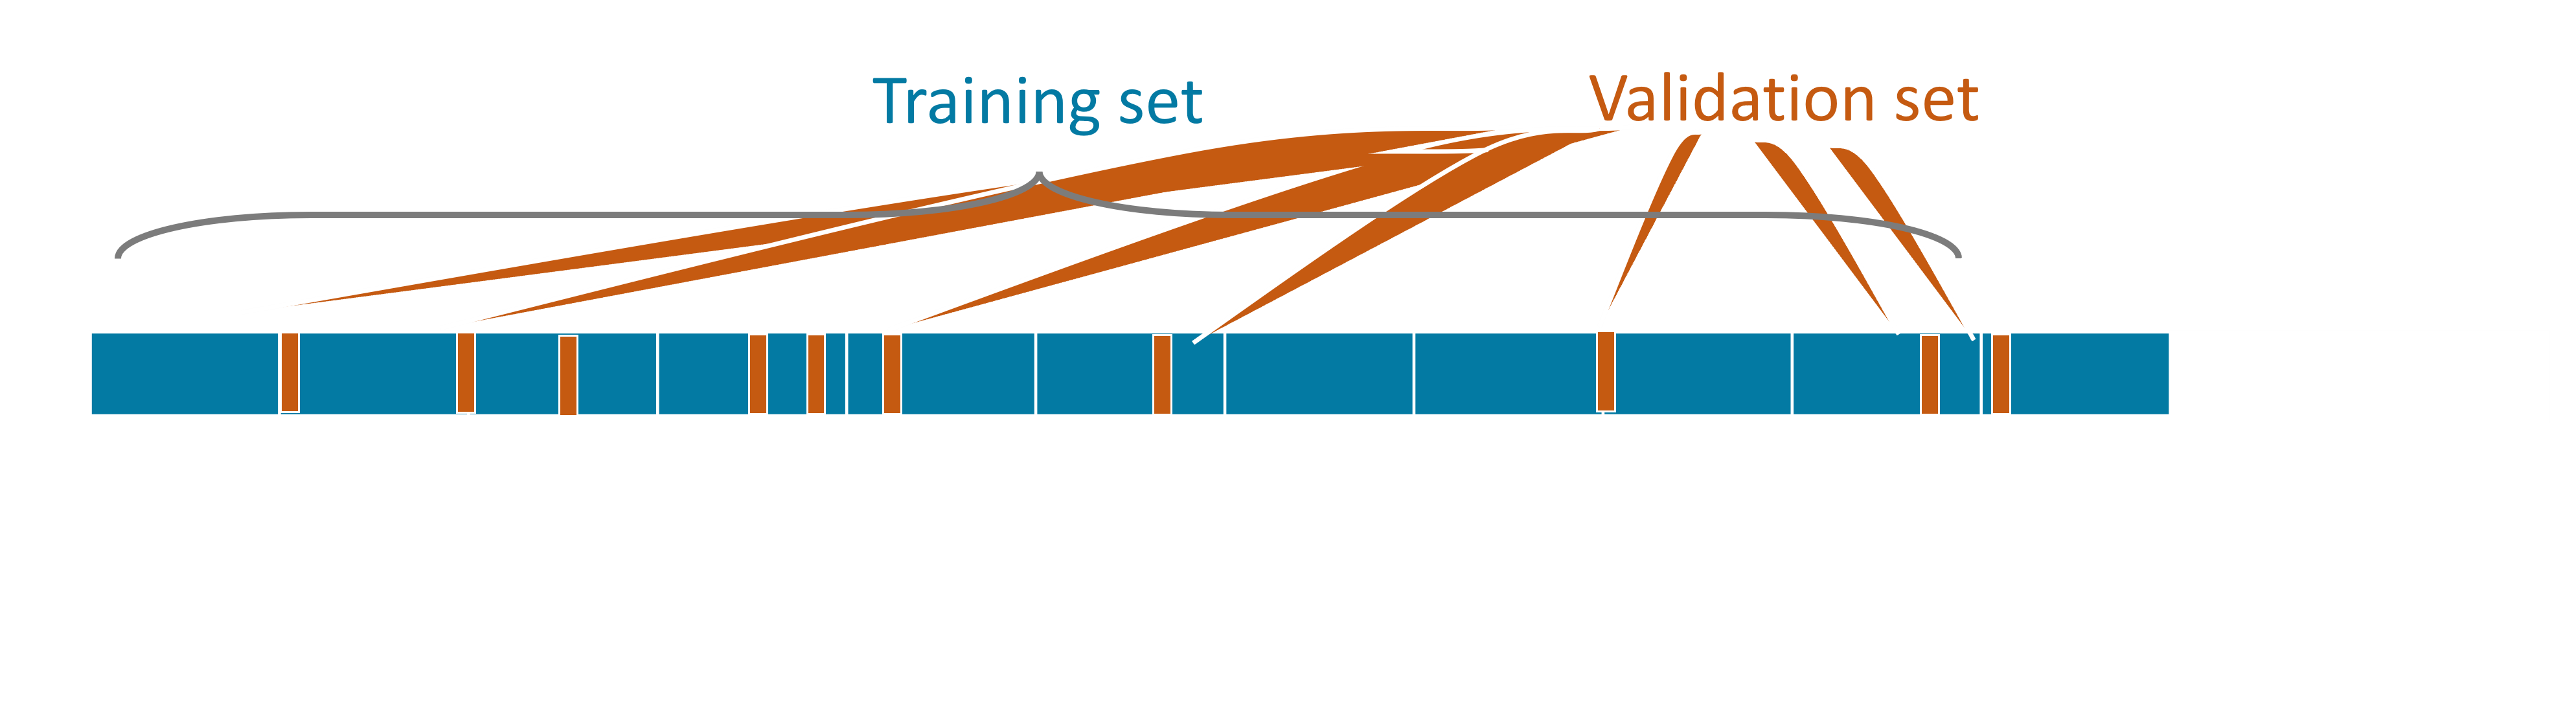
\includegraphics[width = 0.8\textwidth]{ML-Sets5.png}
\end{itemize}
\end{frame}



\begin{frame}
\frametitle{\textcolor{brique}{\textit{Many} different sets!  }}
Using resampling methods to  estimate the error on the prediction
\pause
\begin{itemize}[<+->]\item Cross validation is used to select $m$-(training-validation) sets from the original data set (here again randomly)
\only<2> {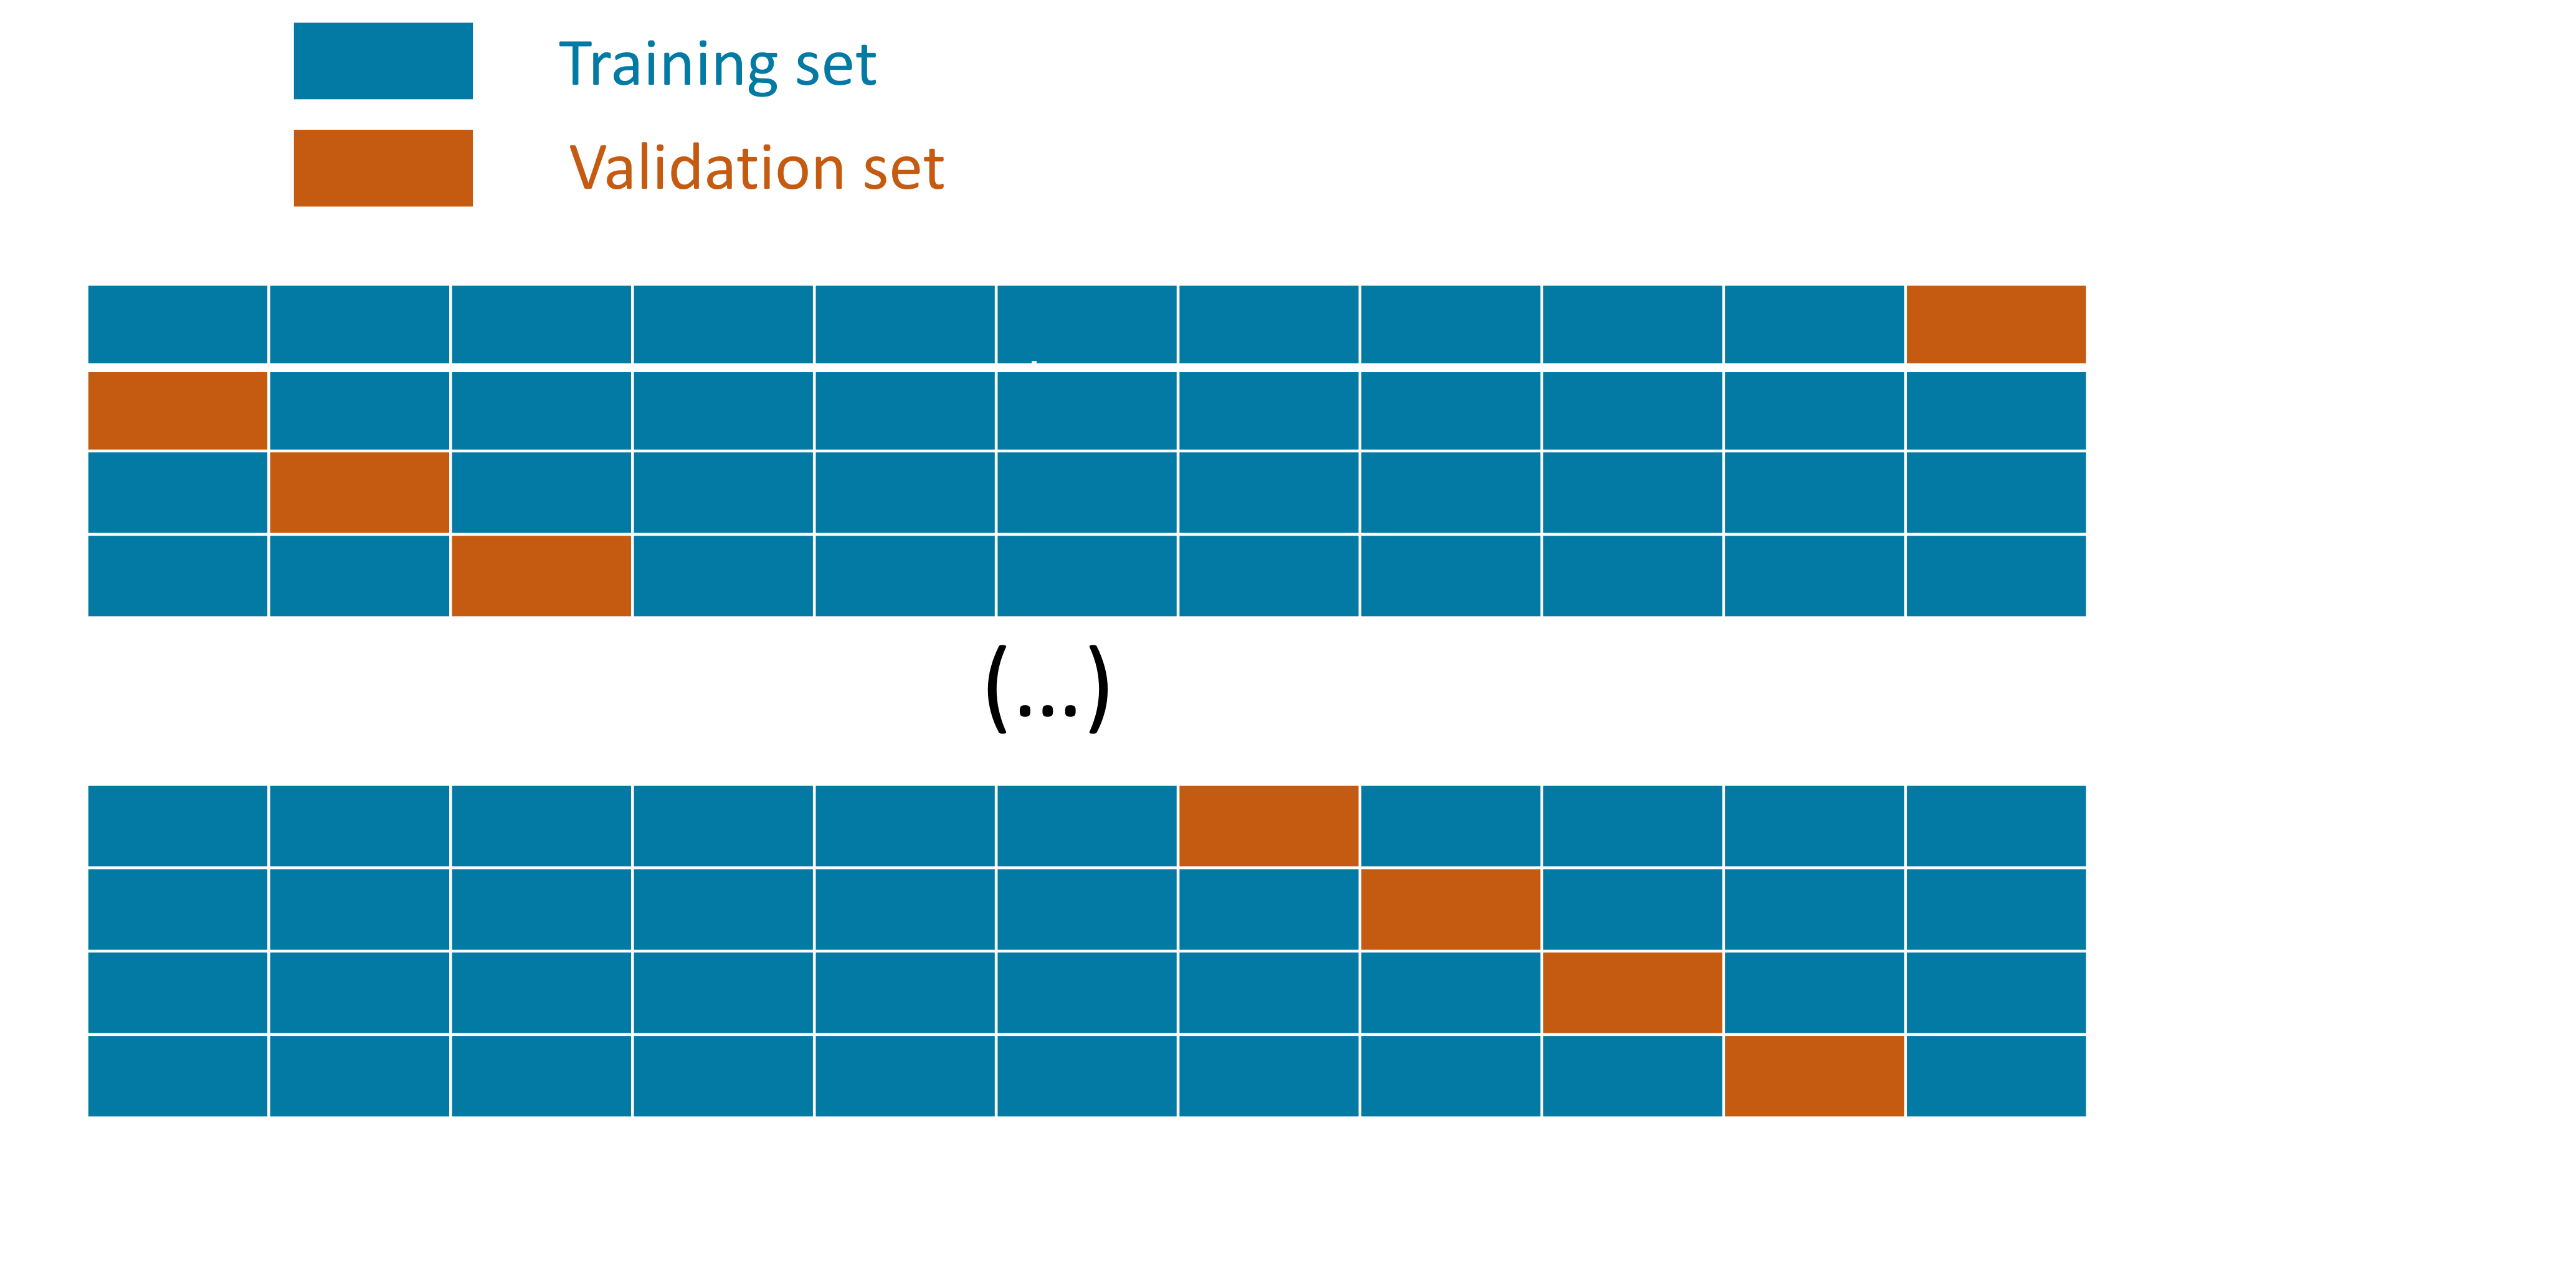
\includegraphics[width = 0.8\textwidth]{CV-Sets1.png}}
\only<3-4> {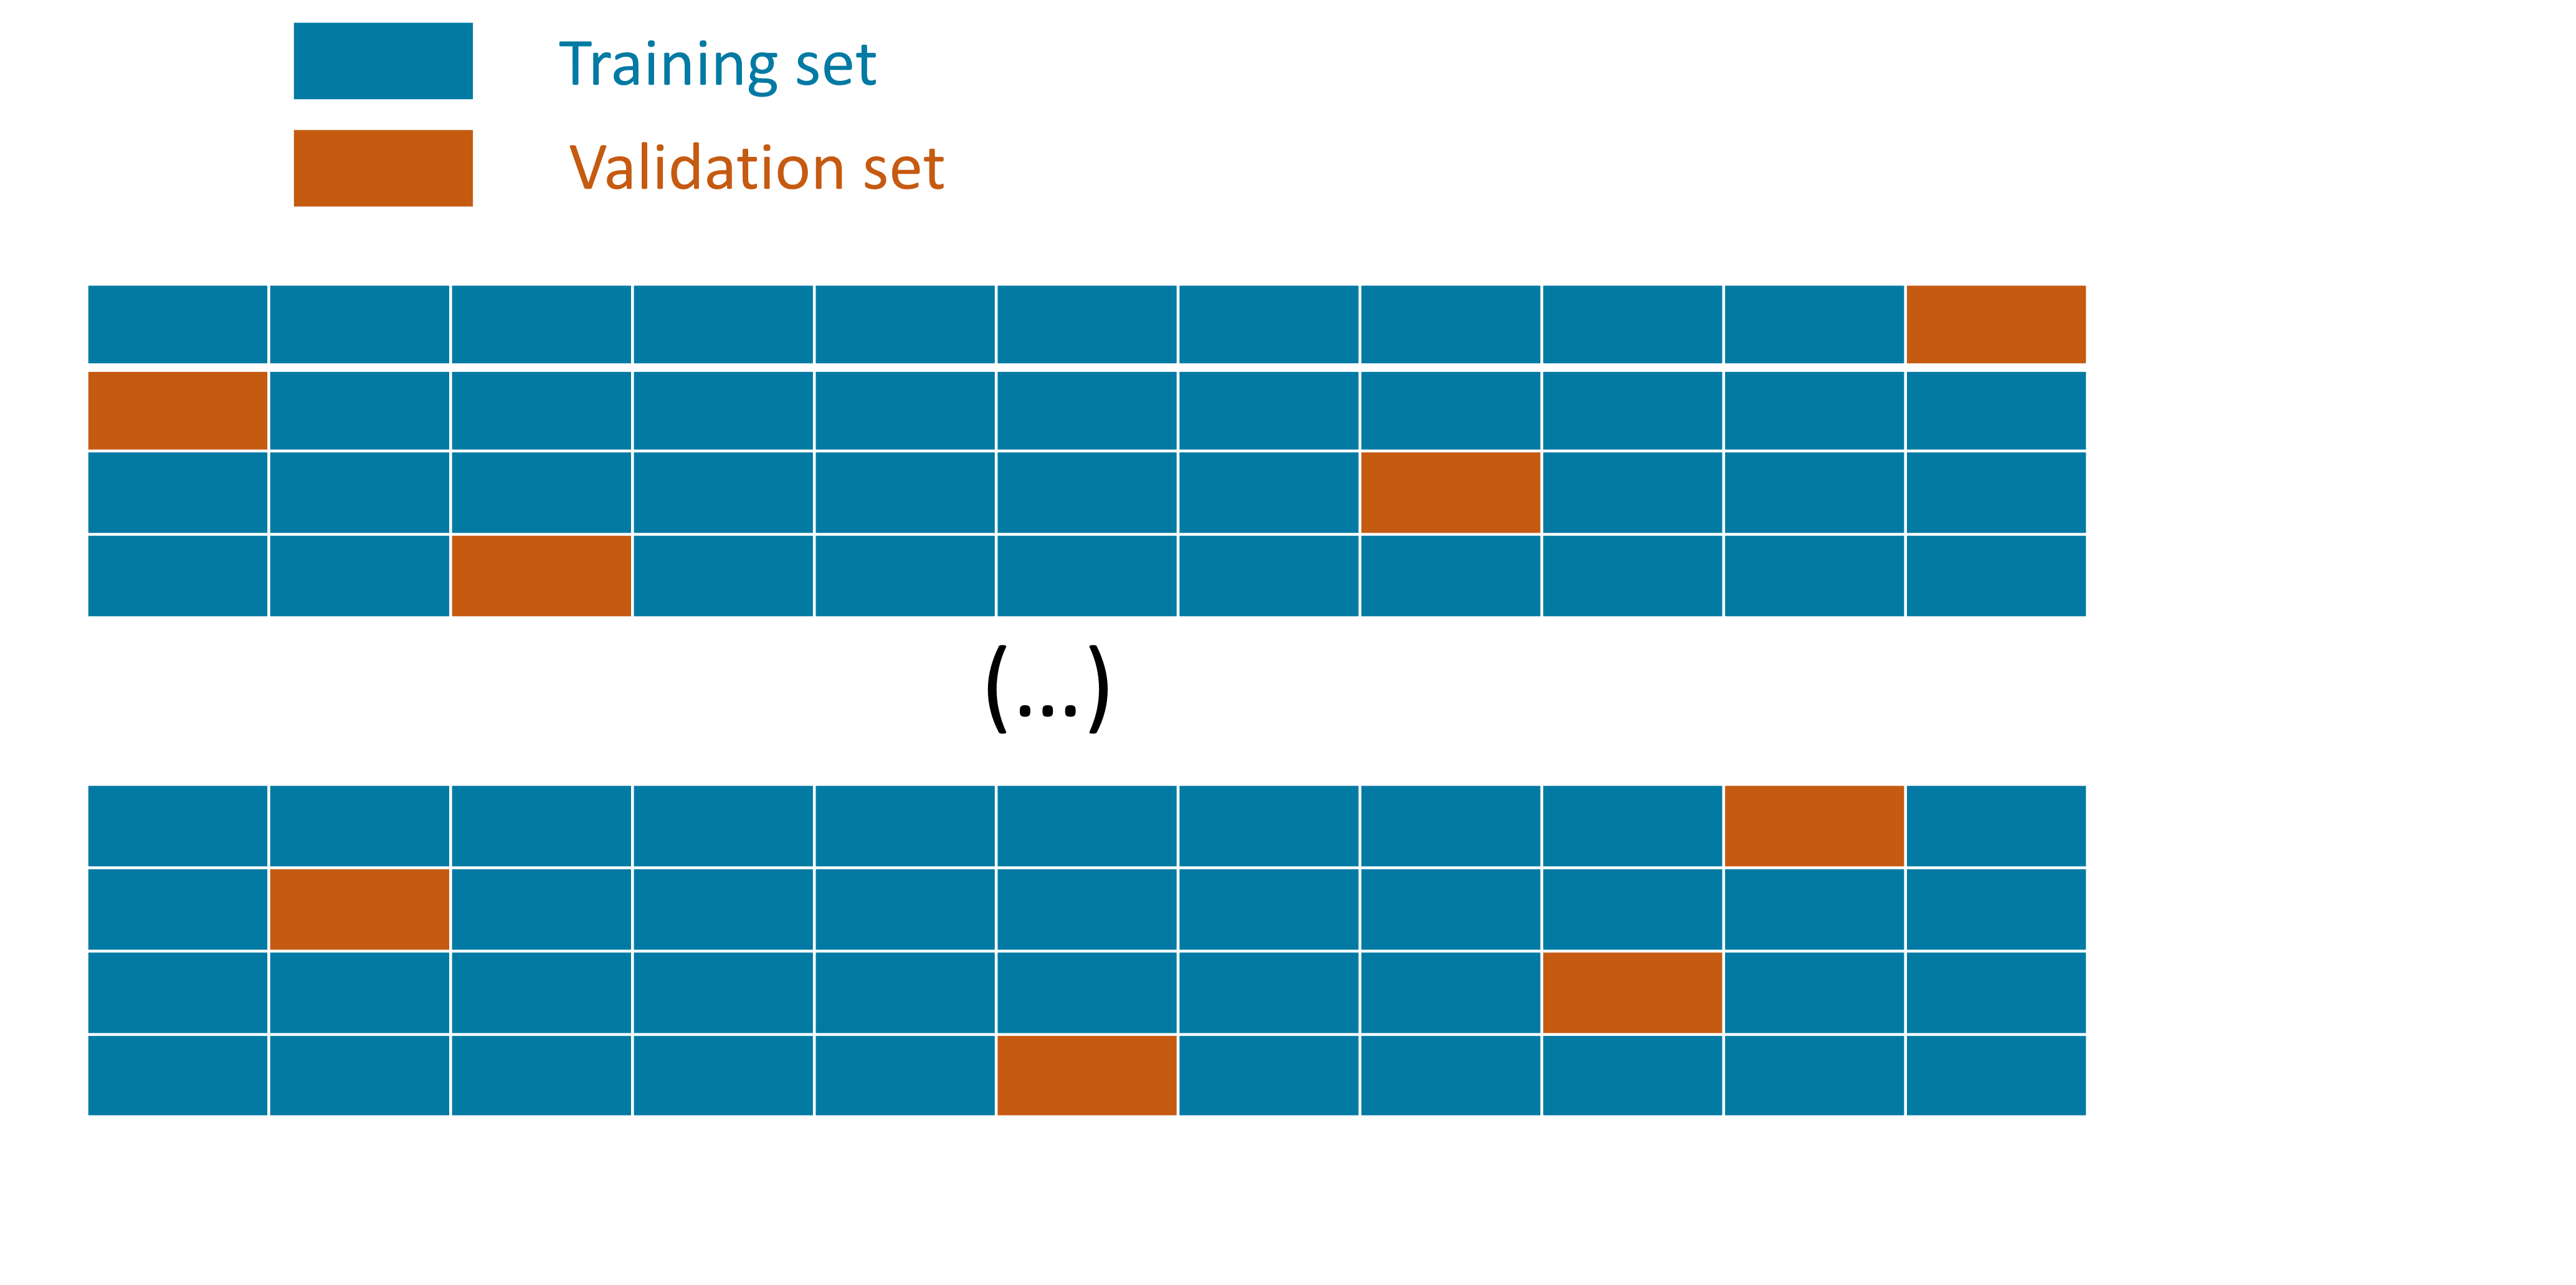
\includegraphics[width = 0.8\textwidth]{CV-Sets2.png}}
 \item[]
\end{itemize}
\end{frame}

\begin{frame}
\frametitle{\textcolor{brique}{\textit{Many} different sets!  }}
\textit{m-fold} Cross-Validation estimates the average prediction error on $m$ different(training-validation) sets
\pause
\begin{itemize}[<+->]
\item For each ($training-validation$) set $j$, one can compute the $MSE_j$ since the true $y$s are known on the validation set!
\item Cross Validation error is then:
 $$ CV_{(m)}  =  \frac{1}{m} \; \sum_ {j=1}^m   MSE_j$$
 \item $CV_{(m)}$ is a good estimate of the prediction error of the model
 \item  $CV_{(m)} $  can serve to select and compare models
 \item[$\hookrightarrow$] Example compute MSE for many models
 %\item In practice $m \in {5, \cdots, 10}$ shows good performances
\end{itemize}
\end{frame}


\section{Wrap-up}

\begin{frame}
\frametitle{\textcolor{brique}{ Wrap-up }}
\pause
\begin{itemize}[<+->]
%\item Machine Learning builds upon "classical" statistics
\item To \textit{understand }the data, we use linear, polynomial, nonparametric models ($k$-NN) or other complex methods (including those for classification)
\item More complex models $\nearrow$ accuracy, but $\rightarrow$ variability (variance) in the estimation
\item  There is a unavoidable  \textbf{bias-variance} trade-off
\item Theory helps understanding but not in choosing the right model
\item The ($train + validation$) sets approach is central in machine learning% The only one that helps in practice
\item[$\hookrightarrow$] In a machine learning framework, the efficiency of the prediction will guide the choices, not the statistical properties! % The only one that helps in practice
\end{itemize}
\end{frame}


\begin{frame} % Cover slide
\frametitle{Definition: Two types of Machine Learning}
\pause
\begin{itemize}[<+->]
  \item We observe \textbf{both} an \textit{outcome} $y$ and \textit{explanatory} variables $x$s
   \item[$\hookrightarrow$] \textbf{Supervised} learning
   \item[] \textit{Most of the examples and applications are supervised learning}
   \item We \textbf{do not} observe an outcome $y$ but\textbf{ only} several $x$s
   \item[$\hookrightarrow$] \textbf{Unsupervised} learning (or \textit{cluster analysis})
  \item[] \textit{More complex models }
 \end{itemize}
\end{frame}

\begin{frame}
\frametitle{\textcolor{brique}{ Tasks for Machine Learning }}
Machine Learning involves several tasks, some are time consuming
\pause
\begin{itemize}[<+->]
    \item Data collection
    \item Data organization
    \item Data cleaning
    \item Data visualization
    \item Data analysis
    \item \textbf{Modeling}
    \item \textbf{Predicting} $\leftarrow$ Focus mostly on this
\end{itemize}
\end{frame}

\begin{frame} % Cover slide
\frametitle{\textcolor{brique}{[Q\&A]}}
\begin{center}
\Large \textcolor{siap}{ Questions?}
\end{center}

\end{frame}


\end{document}
\begin{frame} % Cover slide
\frametitle{ }
\pause
 \begin{itemize}[<+->]
  \item[]
  \item
\end{itemize}
\end{frame}

%%%%%%%%%%%%%%% Last Slide %%%%%%%%%%%%%%%%

\begin{frame}[allowframebreaks]%in case more than 1 slide needed
\frametitle{References}
    {\footnotesize
    %\bibliographystyle{authordate1}
    \bibliographystyle{apalike}
    \bibliography{../../../Visualisation/Visu}
    }
\end{frame}
\end{document}

%\bibliographystyle{authordate1}
%\bibliography{c:/Chris/Visualisation/Visu}
%\end{frame}
